% Design section for AgriConnect documentation
\section{System Design}

\subsection{UML Diagrams}
\begin{figure}[H]
	\centering
	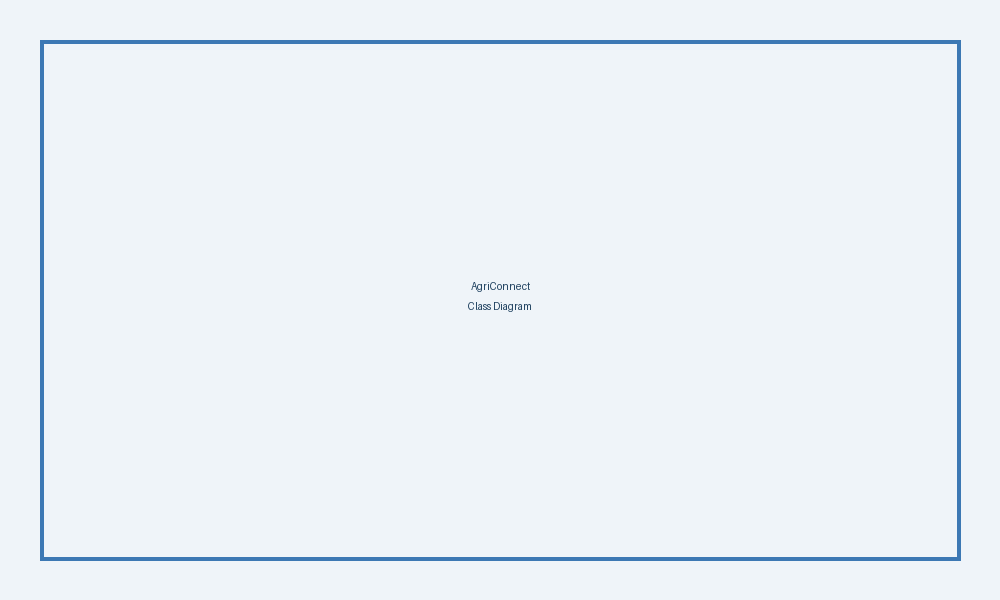
\includegraphics[width=0.7\textwidth]{images/class-diagram.png}
	\caption{Class Diagram}
	\label{fig:class}
\end{figure}

\begin{figure}[H]
	\centering
	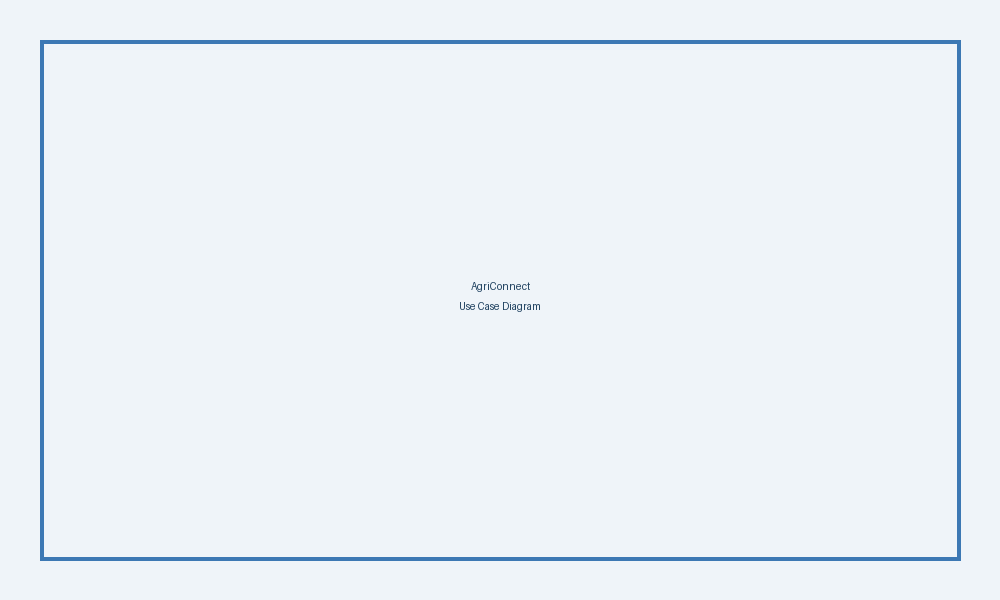
\includegraphics[width=0.7\textwidth]{images/use-case.png}
	\caption{Use Case Diagram}
	\label{fig:usecase}
\end{figure}

\subsection{Database Design}
Core database tables:
\begin{table}[H]
	\centering
	\begin{tabular}{|l|l|}
		\hline
			extbf{Table} & \textbf{Purpose} \\
		\hline
		users & User accounts \\
		farms & Farm information \\
		fields & Field details \\
		activities & Farming activities \\
		listings & Marketplace items \\
		messages & User communications \\
		\hline
	\end{tabular}
	\caption{Database Tables}
	\label{tab:database}
\end{table}

\subsection{API Design}
Key API endpoints:
\begin{verbatim}
POST   /api/auth/register/
POST   /api/auth/login/
GET    /api/farms/
POST   /api/farms/
GET    /api/marketplace/listings/
POST   /api/marketplace/listings/
\end{verbatim}
